\documentclass[border=10pt]{standalone}
\usepackage[svgnames]{xcolor}
\usepackage{amsmath}
\usepackage{pgfplots}
\pgfplotsset{compat=newest}
\usepackage[sfdefault]{FiraSans}
\usepackage{FiraMono}
\renewcommand*\familydefault{\sfdefault}
\begin{document}
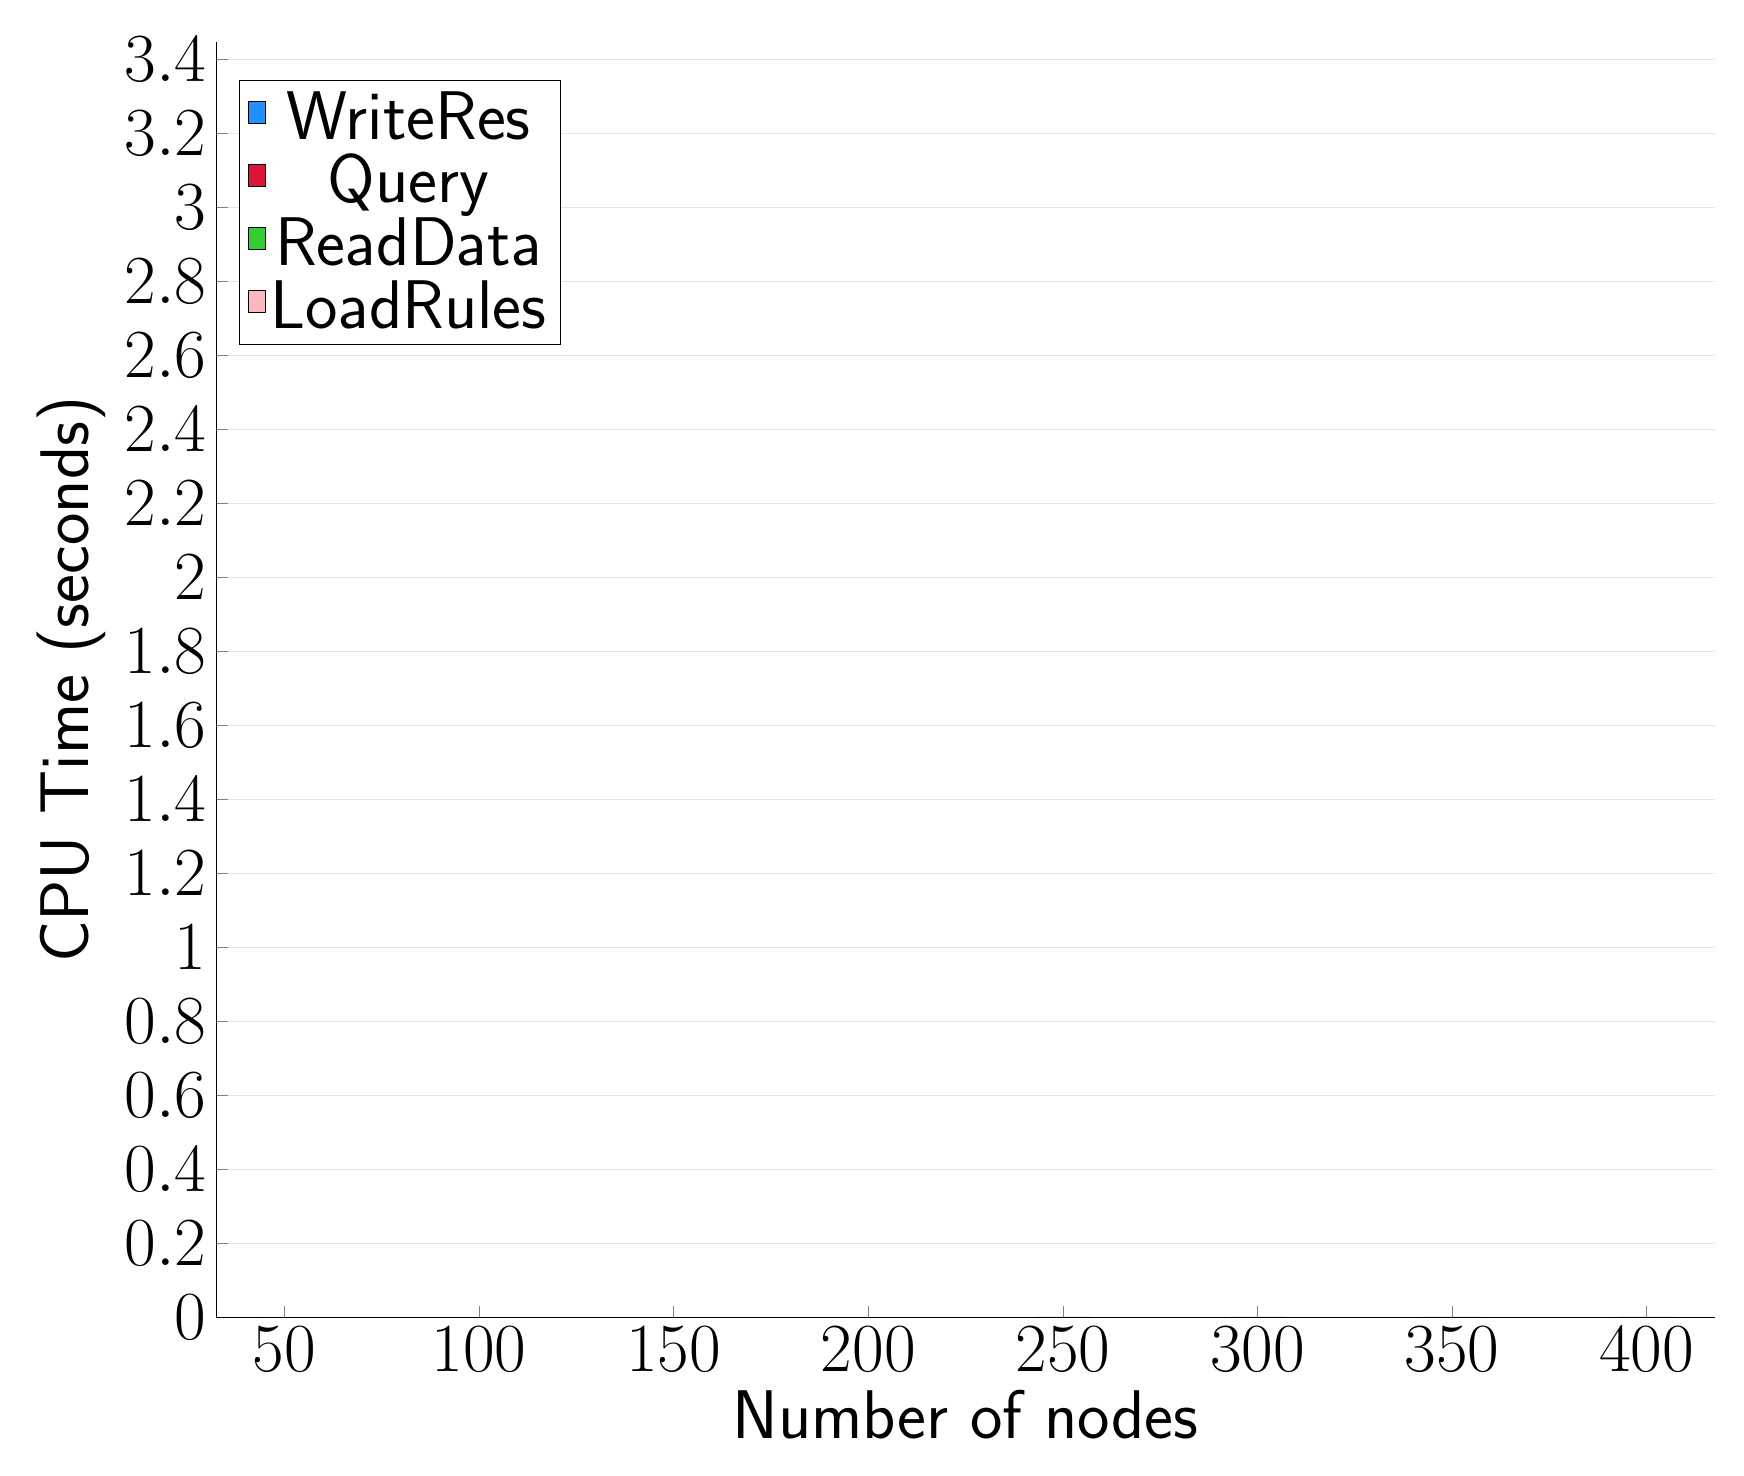
\begin{tikzpicture}
\begin{axis}[
   ybar stacked,
   width=1.7\textwidth,
   bar width=0.7cm,
   ymajorgrids, tick align=inside,
   major grid style={draw=gray!20},
   xtick=data,
   ymin=0, ymax=3.4459999999999997,
   axis x line*=bottom,
   axis y line*=left,
   enlarge x limits=0.05,
   legend style={
       at={(0.23, 0.97)},
       anchor=north east,
       legend columns=1,
       font=\Huge,
   },
   ylabel={CPU Time (seconds)},
   xlabel={Number of nodes},
   label style={font=\Huge},
   tick label style={font=\Huge},
]
\addlegendimage{fill=DodgerBlue, draw=black, line width=0.2pt}
\addlegendentry{WriteRes}
\addlegendimage{fill=Crimson, draw=black, line width=0.2pt}
\addlegendentry{Query}
\addlegendimage{fill=LimeGreen, draw=black, line width=0.2pt}
\addlegendentry{ReadData}
\addlegendimage{fill=LightPink, draw=black, line width=0.2pt}
\addlegendentry{LoadRules}
\addplot +[fill=LightPink, draw=black, line width=0.2pt] coordinates {
(50, 0.0006180999999999999)
(100, 0.0006551999999999997)
(150, 0.0006023999999999997)
(200, 0.0006176000000000004)
(250, 0.0006039)
(300, 0.0006185000000000002)
(350, 0.0006024)
(400, 0.0006145999999999999)
};
\addplot +[fill=LimeGreen, draw=black, line width=0.2pt] coordinates {
(50, 0.00017330000000000042)
(100, 0.0002231000000000001)
(150, 0.00025680000000000006)
(200, 0.0002938999999999999)
(250, 0.00033989999999999986)
(300, 0.00037799999999999997)
(350, 0.0004173000000000002)
(400, 0.00046300000000000003)
};
\addplot +[fill=Crimson, draw=black, line width=0.2pt] coordinates {
(50, 1.3700000000000179e-05)
(100, 2.0100000000000146e-05)
(150, 2.3800000000000036e-05)
(200, 2.829999999999983e-05)
(250, 3.2400000000000306e-05)
(300, 3.950000000000029e-05)
(350, 4.559999999999996e-05)
(400, 5.3200000000000114e-05)
};
\addplot +[fill=DodgerBlue, draw=black, line width=0.2pt] coordinates {
(50, 0.00011319999999999972)
(100, 0.00016119999999999993)
(150, 0.00020309999999999968)
(200, 0.00025250000000000045)
(250, 0.00029769999999999976)
(300, 0.00033709999999999936)
(350, 0.00038769999999999994)
(400, 0.00042450000000000007)
};
\end{axis}
\end{tikzpicture}

\end{document}
